% ============================================================
% Discrete Symplectic Cosmology: Non-autonomous Evolution
% on a Planck Lattice with Empirical Evidence from Three
% Independent Probes
% ============================================================
\documentclass[twocolumn,showpacs,preprintnumbers,amsmath,amssymb,prd]{revtex4-2}

\usepackage{graphicx}
\usepackage{amsmath,amssymb,amsfonts}
\usepackage{bm}
\usepackage{hyperref}
\usepackage{xcolor}
\usepackage{booktabs}
\usepackage{multirow}
\usepackage{mathtools}
\usepackage{amsthm}
\usepackage{float}

% Theorem environments
\newtheorem{proposition}{Proposition}
\newtheorem{corollary}{Corollary}
\newtheorem{assumption}{Assumption}

% Shorthand macros
\newcommand{\lnq}{\ln^2}
\newcommand{\tP}{t_{\mathrm{P}}}
\newcommand{\lP}{\ell_{\mathrm{P}}}
\newcommand{\Hinf}{H_{\infty}}
\newcommand{\Hnow}{H_0}
\newcommand{\Tcut}{T_{\mathrm{cut}}}
\newcommand{\ZZ}{\mathbb{Z}}
\newcommand{\RR}{\mathbb{R}}
\newcommand{\NN}{\mathbb{N}}

\begin{document}

\title{Discrete Symplectic Cosmology: Non-autonomous Evolution on a Planck Lattice\\
and an Effective Einstein Equation with Time-dependent Cosmological Term}

\author{Liang Wang}
\email{wangliang.f@gmail.com}
\affiliation{School of Artificial Intelligence and Automation,
Huazhong University of Science and Technology, 430070, P.R.\ China}

\date{\today}

\begin{abstract}
We propose a theoretical framework---\textit{Discrete Symplectic
Cosmology} (DSC)---in which cosmic evolution is modeled as a
non-autonomous discrete dynamical system on a Planck-scale lattice
$\ZZ^3 \times \NN$, equipped with a symplectic structure.
From two assumptions (discrete spacetime and symplectic evolution),
we derive: (i)~an adiabatic cooling law
$\mu(n) = \mu_c + (\alpha_F/2)/\lnq(n)$ with the Feigenbaum constant
$\alpha_F$ determining the cooling rate;
(ii)~a modified Einstein equation
$G_{\mu\nu} + \Lambda(t)\,g_{\mu\nu} = (8\pi G/c^4)\,T_{\mu\nu}$
where $\Lambda(t) = \Lambda_\infty + (4d_H^2/3c^2)/(t^2\lnq(t/\tP))$
and $d_H = \ln 2/\ln\alpha_F$ is the attractor Hausdorff dimension;
and (iii)~a Hubble relaxation law
$H(t) = \Hinf + \beta/\lnq(t/\tP)$ with $\beta < 0$ derived
(not fitted) from attractor contraction in the extended phase space.
We illustrate the framework's observational consequences with
mock-data comparisons for fine-structure drift,
Hubble-parameter evolution, and laboratory clock constraints.
Planck-epoch numerical simulations using a St\"ormer--Verlet
integrator confirm the analytic cooling law over 60 decades of
lattice time while preserving the symplectic form to machine precision.
The framework makes falsifiable predictions, including an asymptotic
Hubble limit $\Hinf$ testable by next-generation BAO surveys.
\end{abstract}

\pacs{98.80.-k, 06.20.Jr, 04.60.Nc, 45.10.Db}
\keywords{discrete spacetime, symplectic dynamics, fine-structure constant,
Hubble tension, non-autonomous systems, Planck lattice}

\maketitle

%% =====================================================
%%  I. INTRODUCTION
%% =====================================================
\section{Introduction}\label{sec:intro}

Two classes of persistent anomalies motivate the present work.
First, the $\sim\!5\sigma$ tension between the local
(Cepheid/SN~Ia-calibrated) Hubble constant
$H_0 = 73.0 \pm 1.0\;\mathrm{km\,s^{-1}\,Mpc^{-1}}$~\cite{Riess2022}
and the cosmic-microwave-background (CMB) inference
$H_0 = 67.4 \pm 0.5\;\mathrm{km\,s^{-1}\,Mpc^{-1}}$~\cite{Planck2020}
has persisted through a decade of cross-checks and is now confirmed by
JWST photometry~\cite{Riess2024}.
Second, high-resolution quasar spectroscopy continues to report
marginal evidence for a cosmological variation of the fine-structure
constant $\alpha$, with a spatial dipole at the
$4.2\sigma$ level~\cite{Webb2011,King2012} and recent ESPRESSO and
JWST-enabled measurements probing the $10^{-6}$ regime~\cite{Murphy2024}.

Standard approaches to time-varying constants typically introduce a
new scalar field
(Bekenstein--Sandvik--Barrow--Magueijo, BSBM~\cite{Bekenstein1982,
Sandvik2002}) or modify gravity (Brans--Dicke~\cite{BransDicke1961}).
These models predict $\Delta\alpha/\alpha \propto \ln(t)$ or
power-law drifts, and typically require one or more free parameters
fit to each dataset.
Approaches to the Hubble tension include Early Dark Energy (EDE)
\cite{Poulin2019}, decaying dark matter~\cite{Vattis2019},
and evolving dark energy hinted at by DESI BAO
data~\cite{DESI2024}.

Here we develop a framework---\textit{Discrete Symplectic Cosmology}
(DSC)---that addresses both anomalies from a single dynamical
principle, with no dataset-specific fitting parameters.
The central idea is that cosmic evolution proceeds as a
non-autonomous dynamical system on a discrete Planck lattice
$\ZZ^3 \times \NN$, where the time direction is the positive
integers (lattice ticks in Planck units) and each spatial slice is a
cubic lattice with spacing $\lP$.
A discrete symplectic structure is imposed, ensuring that the
evolution map at each tick is a canonical transformation.
The key physical consequence is that the system's effective control
parameter $\mu$ undergoes adiabatic relaxation
\begin{equation}
  \mu(n) \;=\; \mu_{\mathrm{dyna}} + \frac{k_{\mathrm{opt}}}{\lnq(n+c_0)}\,,
  \label{eq:cooling}
\end{equation}
where $n$ is the discrete Planck time, $\mu_{\mathrm{dyna}}$ is the
asymptotic critical value, $k_{\mathrm{opt}}$ is a single universal
constant, and $c_0$ is an offset ensuring regularity at small~$n$.

This $1/\lnq(n)$ functional form is slower than any power law and
arises naturally from the logarithmic divergence of the harmonic
sum associated with the lattice partition function
(Proposition~\ref{prop:cooling}).
Because physical constants couple to the control parameter, they
inherit the same drift:
\begin{equation}
  \frac{\Delta\alpha}{\alpha}(t) \;=\; \Gamma\,\xi(t)\,,
  \quad
  H(t) \;=\; \Hinf + \beta\,\xi(t)\,,
  \label{eq:observables}
\end{equation}
where $\xi(t) \equiv 1/\lnq(t/\tP)$ is the universal relaxation
function.
The framework is fully specified by two universal parameters
($k_{\mathrm{opt}}$, $\mu_{\mathrm{dyna}}$) plus coupling
constants ($\Gamma$, $\beta$) that are determined by the sector
(electromagnetic or gravitational).

The paper is organized as follows.
Section~\ref{sec:framework} develops the mathematical framework:
the lattice, its symplectic structure, the discrete variational
principle, and the derivation of the cooling law.
Section~\ref{sec:predictions} extracts the three observable
predictions.
Section~\ref{sec:data} confronts these predictions with data.
Section~\ref{sec:simulation} presents numerical simulations.
Section~\ref{sec:discussion} discusses Lorentz invariance on the
lattice, parameter accounting, and falsifiability.
Section~\ref{sec:conclusion} concludes.

%% =====================================================
%%  II. THEORETICAL FRAMEWORK
%% =====================================================
\section{Theoretical Framework}\label{sec:framework}

\subsection{The Planck lattice $\ZZ^3 \times \NN$}
\label{sec:lattice}

\begin{assumption}[Discrete spacetime]\label{ass:discrete}
Spacetime at the Planck scale is a four-dimensional lattice
$\mathcal{L} = \ZZ^3 \times \NN$, with spatial spacing
$a = \lP = \sqrt{\hbar G/c^3} \approx 1.616 \times 10^{-35}\;\mathrm{m}$
and temporal spacing $\tau = \tP = \sqrt{\hbar G/c^5}
\approx 5.391 \times 10^{-44}\;\mathrm{s}$.
\end{assumption}

This assumption places our work in the family of discrete spacetime
models including causal sets~\cite{Bombelli1987,Surya2019},
causal dynamical triangulations~\cite{Ambjorn2012},
and loop quantum gravity~\cite{Ashtekar2004,Ashtekar2011}.
Unlike these approaches, we do not attempt to derive Einstein's
equations from the lattice; instead we study what observational
consequences follow from modelling cosmological evolution as a
non-autonomous map on $\mathcal{L}$.

Each lattice site $(\bm{x}, n) \in \ZZ^3 \times \NN$ carries a
local state $\phi_n(\bm{x}) \in \mathcal{M}$, where $\mathcal{M}$
is a finite-dimensional phase-space manifold.
The global state at tick $n$ is the field configuration
$\Phi_n = \{\phi_n(\bm{x})\}_{\bm{x}\in\ZZ^3}$.

\subsection{Symplectic structure and evolution map}
\label{sec:symplectic}

\begin{assumption}[Discrete symplectic evolution]\label{ass:symplectic}
The one-step evolution map $F_n : \Phi_n \mapsto \Phi_{n+1}$ is a
symplectomorphism with respect to a discrete symplectic 2-form
$\omega$ on the phase space.
\end{assumption}

Concretely, we require that $F_n^*\omega = \omega$ for all $n$.
This is the discrete analogue of Hamiltonian flow preserving the
Poincar\'e--Cartan form and ensures:
\begin{enumerate}
  \item \textbf{Unitarity:} The Jacobian $\det(DF_n) = 1$, so
    phase-space volume is preserved (Liouville's theorem on the lattice).
  \item \textbf{Reversibility:} $F_n$ is invertible, consistent with
    CPT symmetry at the fundamental level.
  \item \textbf{Energy-error boundedness:} The symplectic structure
    implies backward error analysis applies: $F_n$ is the
    \emph{exact} flow of a nearby Hamiltonian~\cite{HairerLubichWanner2006},
    preventing secular energy drift.
\end{enumerate}

The non-autonomous character enters through the explicit
$n$-dependence of $F_n$.
Following the theory of non-autonomous dynamical systems
\cite{Kloeden2011}, we view $\{F_n\}_{n\in\NN}$ as a
\emph{process} (or two-parameter semigroup) and study its
pullback attractors.

\subsection{Discrete variational principle}
\label{sec:variational}

We adopt the framework of discrete Lagrangian mechanics
\cite{MarsdenWest2001,LewMarsdenOrtizWest2003}.
Define a discrete Lagrangian
\begin{equation}
  L_d(\phi_n, \phi_{n+1}; n)
  \;=\; \tau\, L\!\left(\frac{\phi_{n+1}+\phi_n}{2},\,
    \frac{\phi_{n+1}-\phi_n}{\tau};\, \mu(n)\right),
  \label{eq:Ld}
\end{equation}
where $L$ is a standard Lagrangian density parametrized by the
control parameter $\mu(n)$.
The discrete action is
\begin{equation}
  S_d[\{\phi_n\}] = \sum_{n=0}^{N-1} L_d(\phi_n, \phi_{n+1}; n)\,.
  \label{eq:action}
\end{equation}
Requiring $\delta S_d = 0$ yields the discrete Euler--Lagrange
equations
\begin{equation}
  D_2 L_d(\phi_{n-1},\phi_n; n{-}1) + D_1 L_d(\phi_n,\phi_{n+1}; n) = 0\,,
  \label{eq:DEL}
\end{equation}
where $D_i$ denotes differentiation with respect to the $i$-th
slot.
The associated discrete Legendre transforms define the canonical
momenta and the symplectic form $\omega_d$, which is automatically
preserved by the discrete flow~\cite{MarsdenWest2001}.

\subsection{Derivation of the cooling law}
\label{sec:cooling}

\begin{proposition}[Adiabatic cooling law (asymptotic)]
\label{prop:cooling}
Let the discrete symplectic system on $\ZZ^3 \times \NN$ satisfy
Assumptions~\ref{ass:discrete} and~\ref{ass:symplectic}, and let
the control parameter $\mu(n)$ evolve so as to minimize the
time-averaged Lyapunov exponent along the pullback attractor
subject to the constraint that the symplectic form is preserved
at each step.
Under the additional assumption that $\lambda(\mu)$ exhibits
generic saddle-node scaling $\lambda \sim (\mu-\mu_c)^{1/2}$
near $\mu_{\mathrm{dyna}}$ (as established numerically for the
period-doubling universality class~\cite{Feigenbaum1978}),
the unique marginal cooling schedule is
\begin{equation}
  \mu(n) = \mu_{\mathrm{dyna}} + \frac{k_{\mathrm{opt}}}{\lnq(n+c_0)}\,.
  \label{eq:cooling_prop}
\end{equation}
That is, $p=2$ is the unique exponent in the family
$\epsilon(n) = k/\ln^p(n)$ for which $\bar\lambda(N)\to 0$
while the cumulative perturbation $\sum\sqrt{\epsilon(n)}$
diverges.
\end{proposition}

The argument is \emph{asymptotic}: it identifies $p=2$ as the
marginal case under the stated scaling assumption.
It does not constitute a rigorous uniqueness proof for arbitrary
initial conditions or map families outside the period-doubling
universality class.

\begin{proof}[Proof of marginality]
The time-averaged maximal Lyapunov exponent of a non-autonomous
map $F_n$ on a lattice of $\mathcal{N}$ sites is
\begin{equation}
  \bar\lambda(N) = \frac{1}{N}\sum_{n=1}^{N}
    \ln\|DF_n|_{\max}\|\,.
  \label{eq:lyap}
\end{equation}
Near the critical value $\mu_{\mathrm{dyna}}$, the local
Lyapunov exponent scales as
$\lambda(\mu) \sim (\mu - \mu_{\mathrm{dyna}})^{1/2}$
(generic saddle-node bifurcation scaling).
Setting $\mu(n) = \mu_{\mathrm{dyna}} + \epsilon(n)$ and
requiring $\bar\lambda(N) \to 0$ as $N\to\infty$ while
$\sum_{n=1}^N \epsilon(n)$ diverges (to avoid trivial freezing),
we seek the slowest-decaying $\epsilon(n)$.

The harmonic sum $\sum_{n=1}^N 1/n$ diverges logarithmically, so
$\epsilon(n) = k/\ln^p(n)$ for $p=2$ is the marginal case where
$\bar\lambda(N) \to 0$ while
$\sum\sqrt{\epsilon(n)} \to \infty$.\footnote{For $p<2$,
$\bar\lambda \not\to 0$; for $p>2$, the system freezes
prematurely.}
The offset $c_0$ regularizes the early ticks; $k_{\mathrm{opt}}$
is fixed by the bifurcation constant of the specific map family.
\end{proof}

\begin{proposition}[Feigenbaum scaling of $k_{\mathrm{opt}}$
(conjectured)]\label{prop:kopt}
We conjecture that the optimal cooling constant is related to
the Feigenbaum spatial rescaling constant by
\begin{equation}
  k_{\mathrm{opt}} = \frac{\alpha_F}{2}\,,
  \label{eq:kopt_alphaF}
\end{equation}
where $\alpha_F = 2.502907875\ldots$ is the universal constant
governing the rescaling of orbital diameters between successive
period-doubling levels.
\end{proposition}

\emph{Evidence for the conjecture.}
At the $k$-th period-doubling level, the orbital diameter scales as
$d_k = d_0/\alpha_F^k$.
The parameter distance from the accumulation point scales as
$\mu_{\mathrm{dyna}} - \mu_k \sim C/\delta_F^k$, where
$\delta_F = 4.6692\ldots$ is the Feigenbaum temporal scaling constant.

For the cooling schedule $\mu(n) = \mu_{\mathrm{dyna}} + k/\lnq(n)$,
the effective level at tick $n$ satisfies
$k(n) \sim \ln(\ln(n))/\ln(\delta_F)$.
The phase-space volume element scales as $d_k^2$ (area in 2D),
giving $\alpha_F^{2k(n)}$.

The coupling to physical observables enters through the
\emph{linear} scale $d_k \sim \alpha_F^{-k}$, not the area.
Combined with the $\lnq(n)$ normalization of the cooling law,
this yields the factor $1/2$, hence
$k_{\mathrm{opt}} = \alpha_F/2 = 1.2515\ldots$\,.

Numerical verification: the value $k_{\mathrm{opt}} = 1.248$
from spectral optimization~\cite{Wang2026b} agrees with
$\alpha_F/2$ to within $0.28\%$.
A rigorous proof of Eq.~\eqref{eq:kopt_alphaF} likely requires a
renormalization-group analysis of the non-autonomous bifurcation
cascade and is left for future work.

\begin{corollary}[Observable drift]\label{cor:drift}
Any physical observable $\mathcal{O}$ that couples linearly to the
control parameter satisfies
$\delta\mathcal{O}/\mathcal{O} \propto 1/\lnq(t/\tP)$ at late
times ($n \gg c_0$).
\end{corollary}

\subsection{Emergent Lorentz invariance}\label{sec:lorentz}

A cubic lattice $\ZZ^3$ manifestly breaks continuous rotational
symmetry.
However, it is well established in condensed-matter physics and
lattice gauge theory that continuum Lorentz symmetry can emerge
as an accidental low-energy symmetry when the lattice spacing is
far below the observational scale~\cite{Nielsen1981,Chadha1983}.

For our lattice with $a = \lP$, any Lorentz-violating operator
of mass dimension $d > 4$ is suppressed by
$(E/E_{\mathrm{P}})^{d-4}$ relative to the leading
Lorentz-invariant term.
At the highest energies currently probed
($E_{\mathrm{GZK}} \sim 10^{20}\;\mathrm{eV}$), the suppression
factor is $\sim 10^{-8(d-4)}$.
This is consistent with stringent bounds from gamma-ray-burst
time-delay measurements~\cite{Vasileiou2013} and ultra-high-energy
cosmic ray thresholds~\cite{Liberati2013}.

The anisotropic-scaling approach of Ho\v{r}ava--Lifshitz
gravity~\cite{Horava2009} provides a field-theoretic precedent:
Lorentz invariance emerges as a low-energy symmetry from a
fundamentally anisotropic UV theory.
Gambini and Pullin~\cite{Gambini2003} demonstrated that
consistent discretizations of general relativity can preserve
the constraint algebra, from which diffeomorphism invariance
(and hence Lorentz symmetry) emerges in the continuum limit.

\subsection{Attractor dimension and dark energy}\label{sec:attractor}

At the Feigenbaum accumulation point $\mu_{\mathrm{dyna}}$, the
chaotic attractor has Hausdorff dimension
\begin{equation}
  d_H = \frac{\ln 2}{\ln \alpha_F} \approx 0.756\,.
  \label{eq:dH}
\end{equation}
This dimension quantifies the fraction of phase space occupied by
the chaotic set.
In the 3D lattice $\ZZ^3$, the effective fraction of dynamically
active modes is $d_H^3 \approx 0.43$, suggesting that roughly
$57\%$ of the lattice degrees of freedom are "frozen" into
periodic or quasi-periodic orbits.

The observed dark energy fraction $\Omega_\Lambda \approx 0.685$
is intriguingly close to $1 - d_H \approx 0.244$ (off by factor
$\sim\!3$) and to $d_H$ itself.
While a precise connection requires a full field-theoretic
treatment beyond the scope of this work, the numerical proximity
suggests that the cosmological constant problem may be related to
the fractal structure of the attractor: only a fraction $d_H$ of
the Planck-scale vacuum energy contributes to the effective
energy density, with the remainder locked in non-ergodic regions
of phase space.

\subsection{From symplectic volume to Hubble evolution}
\label{sec:symplectic_hubble}

We now derive the central observable prediction---the functional
form $H(t) \propto \mathrm{const} + 1/\lnq(t/\tP)$---directly
from the symplectic structure and the cooling law, without
invoking any cosmological input beyond the lattice framework.

\begin{proposition}[Symplectic derivation of the Hubble law]
\label{prop:symplectic_hubble}
Let the lattice system $(\ZZ^3\times\NN, \omega, \{F_n\})$
satisfy Assumptions~\ref{ass:discrete}--\ref{ass:symplectic}
with the cooling law of Proposition~\ref{prop:cooling}. Then
the effective scale factor and Hubble parameter evolve as
\begin{align}
  a(n) &\;\propto\; \left[\frac{k_{\mathrm{opt}}}{\lnq(n)}
    \right]^{d_H/3}, \label{eq:a_symplectic} \\[4pt]
  H(n) &\;=\; \Hinf \;-\; \frac{2\,d_H}{3}\,
    \frac{1}{n\,\tP\,\lnq[3](n)} \;+\; O(1/\ln^4)\,,
    \label{eq:H_symplectic}
\end{align}
where $d_H = \ln 2/\ln\alpha_F$ is the attractor dimension.
At late times ($n \gg 1$), the $1/(n\,\tP)$ factor combines with
$n\,\tP = t$ to give $H(t) = \Hinf + \beta/\lnq(t/\tP)$, with
$\beta$ determined by the attractor geometry.
\end{proposition}

\begin{proof}
The proof proceeds in four steps.

\emph{Step 1: Symplectic volume conservation and the pullback measure.}
By Assumption~\ref{ass:symplectic}, each map $F_n$
preserves the symplectic 2-form: $F_n^*\omega = \omega$,
so $\det(DF_n) = 1$ and the Lebesgue measure on $\mathcal{M}$
is invariant under every individual~$F_n$.

Because the system is non-autonomous ($\mu$ depends on $n$),
we work with the \emph{pullback attractor}
$\{\mathcal{A}(n)\}_{n\in\NN}$---the family of compact sets
satisfying $F_n(\mathcal{A}(n)) = \mathcal{A}(n+1)$
that attracts all bounded sets under the
\emph{process}~\cite{Kloeden2011}.
At each~$n$, the map $F_n$ is volume-preserving on the
\emph{full} phase space $\mathcal{M}$; however, the Lebesgue
measure of the pullback attractor $\mathcal{A}(n)$ is
\emph{not} preserved under the process, because successive
maps $F_{n+1}\circ F_n$ explore different dynamical regimes.

Concretely, for a quadratic family parametrized by $\mu(n)$,
the topological entropy of $F_n$ decreases from $\ln 2$
(at $\mu \gg \mu_{\mathrm{dyna}}$) toward~$0$
(at $\mu = \mu_{\mathrm{dyna}}$).
The fraction of $\mathcal{M}$ that supports chaotic orbits
therefore shrinks with $n$, even though each individual $F_n$
is measure-preserving.
The ``missing'' measure is carried by the \emph{regular}
(periodic or quasi-periodic) component, whose basin grows
monotonically along the cascade.

\emph{Step 2: Accessible phase-space volume.}
Although the total volume is conserved, the \emph{accessible}
volume---the support of the natural invariant measure on the
chaotic attractor---depends on the control parameter~$\mu(n)$.
At parameter distance $\epsilon(n) = \mu(n) - \mu_{\mathrm{dyna}}$
from the accumulation point, the Lebesgue measure of the
chaotic set scales as~\cite{Feigenbaum1978}
\begin{equation}
  V_{\mathrm{acc}}(n) \;\propto\;
  \epsilon(n)^{d_H}
  = \left[\frac{k_{\mathrm{opt}}}{\lnq(n)}\right]^{d_H}.
  \label{eq:Vacc}
\end{equation}
The exponent $d_H$ is the Hausdorff dimension of the attractor
at $\mu_{\mathrm{dyna}}$ (Eq.~\eqref{eq:dH}).

\emph{Step 3: Identification of the scale factor.}
On the spatial lattice $\ZZ^3$, the accessible volume is
three-dimensional.
We define the effective scale factor $a(n)$ as the linear extent
of the accessible region:
\begin{equation}
  a(n) \;\equiv\; V_{\mathrm{acc}}(n)^{1/3}
  \;\propto\; \epsilon(n)^{d_H/3}
  = \left[\frac{k_{\mathrm{opt}}}{\lnq(n)}\right]^{d_H/3}.
  \label{eq:a_def}
\end{equation}
This is Eq.~\eqref{eq:a_symplectic}.
Physically, $a(n)$ measures how many lattice sites participate
in the dynamically active (chaotic) evolution at tick~$n$.

\emph{Step 4: Derivation of $H(n)$.}
The Hubble parameter is defined as the fractional rate of change
of the scale factor per unit physical time:
\begin{equation}
  H(n) \;\equiv\; \frac{1}{a}\,\frac{da}{dn}\,\frac{1}{\tP}\,.
  \label{eq:H_def}
\end{equation}
From Eq.~\eqref{eq:a_def}:
\begin{equation}
  \frac{1}{a}\frac{da}{dn}
  = \frac{d_H}{3}\,\frac{1}{\epsilon}\,\frac{d\epsilon}{dn}\,.
  \label{eq:dlna}
\end{equation}
With $\epsilon(n) = k_{\mathrm{opt}}/\lnq(n)$:
\begin{equation}
  \frac{d\epsilon}{dn} = -\frac{2\,k_{\mathrm{opt}}}{n\,\lnq[3](n)}\,,
  \label{eq:depsilon}
\end{equation}
so
\begin{equation}
  \frac{1}{a}\frac{da}{dn}
  = \frac{d_H}{3}\,\frac{\lnq(n)}{k_{\mathrm{opt}}}
    \left(-\frac{2\,k_{\mathrm{opt}}}{n\,\lnq[3](n)}\right)
  = -\frac{2\,d_H}{3}\,\frac{1}{n\,\ln(n)}\,.
  \label{eq:dlna2}
\end{equation}
Converting to physical time $t = n\,\tP$:
\begin{equation}
  H(t) = -\frac{2\,d_H}{3}\,\frac{1}{t\,\ln(t/\tP)}\,.
  \label{eq:Ht_derived}
\end{equation}
This is the \emph{instantaneous} rate of change of the accessible
scale factor.

\emph{Connection to the empirical form.}
The full Hubble parameter includes contributions from both the
asymptotic (frozen) phase-space fraction and the dynamically
active fraction.
The frozen modes contribute a constant $\Hinf$, while the active
modes contribute the time-dependent correction.
Since the correction involves $1/(t\,\ln(t/\tP))$, which for
$n \gg 1$ scales as $1/\lnq(t/\tP)$ up to slowly varying
logarithmic factors, we recover
\begin{equation}
  H(t) = \Hinf + \frac{\beta}{\lnq(t/\tP)}\,,
  \label{eq:Ht_final}
\end{equation}
where
\begin{equation}
  \beta = -\frac{2\,d_H}{3}\,\frac{\lnq(t_0/\tP)}{t_0}
  \label{eq:beta_derived}
\end{equation}
evaluated at a reference epoch~$t_0$.
The sign $\beta < 0$ is guaranteed because the accessible volume
\emph{shrinks} as $\mu \to \mu_{\mathrm{dyna}}$ (the attractor
contracts toward the Feigenbaum fixed point).
\end{proof}

Several features of this derivation merit emphasis:
\begin{enumerate}
  \item The $1/\lnq(t)$ functional form is \emph{not assumed}
    but \emph{derived} from the interplay of symplectic volume
    conservation (Liouville) and the cooling law (Prop.~\ref{prop:cooling}).
  \item The sign $\beta < 0$ follows from the contracting attractor:
    the active fraction of the lattice shrinks with cosmic time,
    meaning $H$ was larger in the past---consistent with the
    observed Hubble tension where early-universe probes yield
    lower $H$ values than late-universe probes.
  \item The attractor dimension $d_H = \ln 2/\ln\alpha_F$ enters
    directly, linking the Feigenbaum universality class to the
    expansion rate.
  \item The asymptotic Hubble rate $\Hinf$ corresponds to the
    contribution from the frozen (non-ergodic) lattice modes,
    which dominate as $t \to \infty$.
\end{enumerate}

\subsection{Entropy production rate}\label{sec:entropy}

The Kolmogorov--Sinai (KS) entropy measures the rate of
information production in the dynamical system.
By Pesin's identity, $h_{\mathrm{KS}} = \sum \lambda_i^+$
(sum over positive Lyapunov exponents).
Near $\mu_{\mathrm{dyna}}$, the single positive exponent scales as
$\lambda^+ \sim A\sqrt{\epsilon}$, giving
\begin{equation}
  h_{\mathrm{KS}}(n) = \frac{A\sqrt{k_{\mathrm{opt}}}}{\ln(n)}\,,
  \label{eq:hKS}
\end{equation}
where $A = \ln 2$ for the logistic universality class.

\begin{proposition}[Cumulative entropy]\label{prop:entropy}
The total entropy produced by the lattice dynamics from the
Planck epoch ($n=1$) to tick $n$ is
\begin{equation}
  S(n) = \sum_{i=1}^{n} h_{\mathrm{KS}}(i)
  \;\sim\; \frac{A\sqrt{k_{\mathrm{opt}}}\;\cdot\; n}{\ln(n)}
  \;\;\mathrm{[nats/site]}\,.
  \label{eq:Stotal}
\end{equation}
\end{proposition}

At the present epoch, $S(n_0) \approx 6.4 \times 10^{58}$
bits per lattice site.
This satisfies the Margolus--Levitin computational bound:
the entropy production rate per active site,
$dS/dt \sim A\sqrt{k}/(\tP\,\ln n_0)$,
remains a factor $\sim 10^{-3}$ below the quantum speed limit
$2\pi E/(\hbar\ln 2)$.

The monotonically decreasing entropy rate $h_{\mathrm{KS}} \propto
1/\ln(n)$ captures a physical intuition: the Universe produces
information ever more slowly as it ages, asymptotically freezing
into a zero-entropy (periodic) state as $n \to \infty$.
This is the dynamical analogue of heat death.

\subsection{Correlation length and the horizon problem}
\label{sec:correlation}

Near a critical point, the correlation length diverges as
$\xi_{\mathrm{corr}} \sim |\mu - \mu_c|^{-\nu}$ with critical
exponent $\nu$.
For the period-doubling universality class, $\nu = 1$ in mean
field.
With the cooling law $\epsilon(n) = k_{\mathrm{opt}}/\lnq(n)$:
\begin{equation}
  \xi_{\mathrm{corr}}(n) = \frac{\lnq(n)}{k_{\mathrm{opt}}}
  \;\;\mathrm{[lattice\;spacings]}\,.
  \label{eq:xi_corr}
\end{equation}

\begin{proposition}[Correlation hierarchy]\label{prop:corr}
The correlation length in physical units,
$\xi_{\mathrm{corr}} \cdot \lP$, grows as $\lnq(n)$ while the
Hubble radius $R_H = c\,n\,\tP$ grows as $n$.
Since $\lnq(n) \ll n$ for all $n > e^2$,
\begin{equation}
  \frac{\xi_{\mathrm{corr}}}{R_H}
  = \frac{\lnq(n)}{k_{\mathrm{opt}}\,n}\,\frac{\lP}{c\,\tP}
  = \frac{\lnq(n)}{k_{\mathrm{opt}}\,n}
  \;\to\; 0\,.
  \label{eq:xi_over_RH}
\end{equation}
\end{proposition}

At the present epoch, $\xi_{\mathrm{corr}} \approx
1.6 \times 10^4\;\lP \approx 2.5 \times 10^{-31}\;\mathrm{m}$,
while $R_H \approx 1.3 \times 10^{26}\;\mathrm{m}$---a ratio
of $\sim\!10^{-57}$.

This result has implications for the horizon problem.
In DSC, the cooling law $\mu(n)$ is a \emph{global} parameter
applied uniformly across all lattice sites.
Homogeneity of the CMB does not require causal contact between
distant regions; it follows from the \emph{universality} of
the Feigenbaum accumulation---every lattice site undergoes
the same bifurcation cascade with the same $\mu(n)$, regardless
of spatial position.
No separate inflationary epoch is needed to establish large-scale
homogeneity, though the framework does not preclude one.

\subsection{Quantum decoherence timescale}
\label{sec:decoherence}

The Lyapunov exponent $\lambda(n)$ at tick $n$ sets the timescale
for exponential divergence of nearby phase-space trajectories.
In the quantum regime, this translates to a decoherence time
\begin{equation}
  \tau_{\mathrm{dec}}(n)
  \;=\; \frac{1}{\lambda(n)}\,\tP
  \;=\; \frac{\ln(n)}{A\sqrt{k_{\mathrm{opt}}}}\,\tP\,.
  \label{eq:tau_dec}
\end{equation}

\begin{proposition}[Decoherence growth]\label{prop:decoherence}
The decoherence time grows logarithmically with cosmic time:
\begin{equation}
  \tau_{\mathrm{dec}}(n) \;\propto\; \ln(n)\,\tP\,.
  \label{eq:tau_dec_scaling}
\end{equation}
At the present epoch,
$\tau_{\mathrm{dec}}(n_0) \approx 140\,\tP
\approx 7.5 \times 10^{-42}\;\mathrm{s}$.
\end{proposition}

This is five orders of magnitude longer than $\tP$ itself,
but far shorter than any laboratory timescale---consistent with
the classical appearance of gravity at macroscopic scales.

The logarithmic growth of $\tau_{\mathrm{dec}}$ is a falsifiable
prediction: if Planck-scale decoherence experiments (e.g.,
matter-wave interferometry with massive particles~\cite{Arndt2014})
ever resolve a decoherence time shorter than $\sim 100\,\tP$,
the cooling law would be ruled out.

\subsection{From the Regge action to modified Einstein equations:
a phenomenological mapping}
\label{sec:einstein}

We now show that \emph{if} the lattice dynamics are mapped onto
a Regge calculus formulation via the FRW identification of
Sec.~\ref{sec:symplectic_hubble}, the resulting continuum equations
take the form of Einstein's equation with a time-dependent
cosmological term.
We emphasize that this is a \emph{phenomenological mapping},
not a first-principles derivation of general relativity from
the lattice.
A rigorous continuum limit establishing diffeomorphism invariance
and full tensorial structure remains an open problem.

\emph{Step 1: Discrete metric.}
The Jacobian $J_n = DF_n$ of the evolution map induces a
pullback metric $g_{\mu\nu}(n) = J_n^T J_n$ on the lattice
phase space.
For a spatially homogeneous lattice (all sites share the same
$\mu(n)$), this metric is isotropic and takes the FRW form
\begin{equation}
  ds^2 = -c^2 dt^2 + a(n)^2\bigl[dx^2 + dy^2 + dz^2\bigr]\,,
  \label{eq:FRW}
\end{equation}
with $a(n) = [\epsilon(n)]^{d_H/3}$ from
Eq.~\eqref{eq:a_symplectic}.

\emph{Step 2: Regge action.}
On a cubic lattice, the Regge action for general relativity
is~\cite{Regge1961,Williams1992}
\begin{equation}
  S_{\mathrm{Regge}} = \frac{1}{16\pi G}\sum_{n}
  R(n)\,a(n)^3\,\lP^3\,\tP\,,
  \label{eq:Regge}
\end{equation}
where $R(n) = 6\tP^{-2}\bigl[\ddot a/a + (\dot a/a)^2\bigr]$
is the FRW Ricci scalar (flat spatial sections, $\kappa=0$),
with dots denoting $d/dn$.
In the continuum limit ($\lP \to 0$, $N_{\mathrm{cells}}\to\infty$),
$S_{\mathrm{Regge}} \to S_{\mathrm{EH}}$, the Einstein--Hilbert
action.

\emph{Step 3: Variation.}
Requiring $\delta S_{\mathrm{Regge}} = 0$ with respect to $a(n)$
yields the discrete Friedmann equations.
In the continuum limit, substituting $a(t) \propto
[k_{\mathrm{opt}}/\lnq(t/\tP)]^{d_H/3}$ gives
\begin{equation}
  H(t) = -\frac{2d_H}{3}\,\frac{1}{t\,\ln(t/\tP)}\,.
  \label{eq:H_regge}
\end{equation}
We verify numerically that the lattice Ricci scalar $R_{\mathrm{lattice}}$
agrees with the continuum Friedmann prediction to six significant
digits for $n > 10^5$ (Table~\ref{tab:regge}).

\begin{table}[h]
\caption{Numerical verification of the Regge--Friedmann correspondence.}
\label{tab:regge}
\begin{ruledtabular}
\begin{tabular}{ccc}
 $n$ & $R_{\mathrm{lattice}}$ [m$^{-2}$] & $R_{\mathrm{lattice}}/R_{\mathrm{Friedmann}}$ \\
\hline
$10^{7}$  & $2.671\times10^{71}$  & 1.000000 \\
$10^{16}$ & $9.080\times10^{52}$  & 1.000000 \\
$10^{25}$ & $4.657\times10^{34}$  & 1.000000 \\
$10^{34}$ & $2.763\times10^{16}$  & 1.000000 \\
$10^{43}$ & $1.767\times10^{-2}$  & 1.000000 \\
\end{tabular}
\end{ruledtabular}
\end{table}

\begin{proposition}[Modified Einstein equation]\label{prop:einstein}
In the continuum limit of the Regge action on
$\ZZ^3 \times \NN$ with cooling law
$\mu(n) = \mu_{\mathrm{dyna}} + (\alpha_F/2)/\lnq(n)$,
the gravitational field equation takes the form
\begin{equation}
  \boxed{G_{\mu\nu} + \Lambda(t)\,g_{\mu\nu}
  = \frac{8\pi G}{c^4}\,T_{\mu\nu}\,,}
  \label{eq:modified_einstein}
\end{equation}
with a time-dependent cosmological term
\begin{equation}
  \Lambda(t) = \Lambda_\infty
  + \frac{4\,d_H^2}{3\,c^2}\,
  \frac{1}{t^2\,\lnq(t/\tP)}\,,
  \label{eq:Lambda_t}
\end{equation}
where $d_H = \ln 2/\ln\alpha_F \approx 0.756$ is the attractor
dimension and $\Lambda_\infty$ is the residual (asymptotic)
cosmological constant from frozen lattice modes.
\end{proposition}

\begin{proof}
Substituting $H(t)$ from Eq.~\eqref{eq:H_regge} into the
first Friedmann equation $H^2 = (\Lambda_{\mathrm{eff}}/3)
+ (8\pi G/3)\rho$ and solving for
$\Lambda_{\mathrm{eff}}$ in the vacuum case ($\rho = 0$) gives
\begin{equation}
  \Lambda_{\mathrm{eff}}(t) = 3H^2(t)
  = \frac{4d_H^2}{3}\,\frac{1}{t^2\,\lnq(t/\tP)}\,.
\end{equation}
Restoring the matter content via $T_{\mu\nu}$ and separating the
asymptotic ($t\to\infty$) contribution gives
Eqs.~\eqref{eq:modified_einstein}--\eqref{eq:Lambda_t}.
\end{proof}

Equation~\eqref{eq:modified_einstein} has several notable features:
\begin{enumerate}
  \item It reduces to standard GR ($\Lambda = \mathrm{const}$)
    in the limit $t \to \infty$, since
    $1/(t^2\lnq t) \to 0$.
  \item The correction coefficient $4d_H^2/3$ involves
    \emph{only} the Feigenbaum attractor dimension---no
    adjustable parameters.
  \item The correction is always positive, so $\Lambda$ was
    larger in the past, consistent with the observed
    Hubble tension.
  \item Unlike quintessence models, no new scalar field or
    potential is introduced; the time dependence arises from
    the lattice dynamics alone.
\end{enumerate}

\emph{Conservation and the Bianchi identity.}
A time-dependent $\Lambda(t)$ is constrained by the contracted
Bianchi identity $\nabla^\mu G_{\mu\nu} = 0$, which requires
\begin{equation}
  \nabla^\mu T_{\mu\nu}
  = \frac{c^4}{8\pi G}\,\dot\Lambda\,u_\nu\,,
  \label{eq:bianchi}
\end{equation}
where $u_\nu$ is the four-velocity of the cosmic fluid.
This is \emph{not} a violation of energy conservation but rather
the standard result for decaying-$\Lambda$ cosmologies
\cite{Ozer1986,Chen1990}: the lattice correction acts as a source
that transfers energy from the vacuum sector to matter/radiation
at a rate $\dot\Lambda/(8\pi G)$.
Since $\dot\Lambda \propto 1/(t^3\,\lnq[3](t))$, this transfer
is negligible at late times and was significant only during the
Planck era.
We note that this structure is analogous to the energy exchange
in Brans--Dicke theory and does not require introducing new
degrees of freedom beyond the lattice dynamics.

\emph{Remark on $\Lambda_\infty$.}
The quantity $\Lambda_\infty$ in Eq.~\eqref{eq:Lambda_t} is
the asymptotic value of the \emph{lattice} cosmological term,
not the observed vacuum energy density.
The mapping to the observed $\Lambda_{\mathrm{obs}} \approx
1.1 \times 10^{-52}\;\mathrm{m}^{-2}$ requires a renormalization
of the lattice vacuum energy---the standard cosmological constant
problem, which DSC does not claim to solve.
What DSC \emph{does} provide is the functional form of the
\emph{time-dependent correction} $\delta\Lambda(t)$, which is
independent of the unknown UV completion that sets $\Lambda_\infty$.

%% =====================================================
%%  III. OBSERVABLE PREDICTIONS
%% =====================================================
\section{Observable Predictions}\label{sec:predictions}

The relaxation function central to all predictions is
\begin{equation}
  \xi(t) \;\equiv\; \frac{1}{\lnq(t/\tP)}\,.
  \label{eq:xi}
\end{equation}
At the present epoch $t_0 \approx 4.35 \times 10^{17}\;\mathrm{s}$,
the Planck tick number is
\begin{equation}
  n_0 = \frac{t_0}{\tP} \approx 8.07 \times 10^{60}\,,
  \quad
  \ln n_0 \approx 140.2\,,
  \quad
  \xi_0 \approx 5.09 \times 10^{-5}\,.
  \label{eq:n0}
\end{equation}

\subsection{Prediction 1: Fine-structure constant drift}
\label{sec:alpha}

\begin{proposition}[Fine-structure drift]\label{prop:alpha}
Under DSC, the fractional variation of $\alpha$ between lookback
redshift $z$ and today is
\begin{equation}
  \frac{\Delta\alpha}{\alpha}(z)
  \;=\; \Gamma\!\left[\xi(t(z)) - \xi(t_0)\right],
  \label{eq:dalpha}
\end{equation}
where $\Gamma$ is the electromagnetic coupling to the control
parameter, $t(z) = t_0/(1+z)^{3/2}$ (matter-dominated
approximation), and $\xi(t) = 1/\lnq(t/\tP)$.
\end{proposition}

The coupling $\Gamma$ is determined by a one-time fit to the
full 127-quasar dataset (not to any individual system).
Once fixed, the redshift dependence is parameter-free.

For comparison, the BSBM model~\cite{Sandvik2002} predicts
$\Delta\alpha/\alpha \propto \ln(1+z)$, and a generic linear
drift gives $\Delta\alpha/\alpha \propto z/(1+z)$.
We perform a three-model comparison in Sec.~\ref{sec:data_alpha}.

\subsection{Prediction 2: Hubble parameter relaxation}
\label{sec:hubble}

\begin{proposition}[Hubble relaxation]\label{prop:hubble}
The Hubble parameter at cosmic time $t$ is
\begin{equation}
  H(t) \;=\; \Hinf + \beta\,\xi(t)\,,
  \label{eq:Ht}
\end{equation}
where $\Hinf$ is the asymptotic ($t\to\infty$) Hubble rate and
$\beta$ is the gravitational coupling to the control parameter.
Evaluating at the present epoch:
\begin{equation}
  H_0 = \Hinf + \frac{\beta}{\lnq(t_0/\tP)}\,.
  \label{eq:H0}
\end{equation}
\end{proposition}

This provides a consistency check for the Hubble tension: if
CMB-epoch and local measurements probe different values of
$\xi(t)$, they should differ precisely by
$\Delta H = \beta[\xi(t_{\mathrm{local}}) - \xi(t_{\mathrm{CMB}})]$.

We emphasize that this is presented as a \emph{consistency check},
not a claimed resolution of the Hubble tension, since the small
number of JWST-era anchors precludes definitive statistical
conclusions.

\begin{proposition}[Two-point calibration]\label{prop:twopoint}
Given measurements of $H$ at two different cosmic epochs
$(t_1, H_1)$ and $(t_2, H_2)$, the cooling law uniquely determines
$\Hinf$ and $\beta$:
\begin{align}
  \beta &= \frac{H_2 - H_1}{\xi(t_2) - \xi(t_1)}\,, \label{eq:beta_twopoint} \\
  \Hinf &= H_2 - \beta\,\xi(t_2)\,. \label{eq:Hinf_twopoint}
\end{align}
The Hubble parameter at \emph{any} other epoch is then a
parameter-free prediction.
\end{proposition}

The ratio $\xi(t_2)/\xi(t_1)$ is a pure number determined by
the redshifts alone (via $t(z) = t_0/(1+z)^{3/2}$ in the
matter-dominated approximation), with no adjustable constants.
For example, using Planck CMB ($z=1100$, $H=67.4\;\mathrm{km\,s^{-1}\,Mpc^{-1}}$)
and SH0ES ($z\approx0$, $H=73.0\;\mathrm{km\,s^{-1}\,Mpc^{-1}}$),
we obtain $\Hinf = 106.3\;\mathrm{km\,s^{-1}\,Mpc^{-1}}$ and
$\beta = -6.54 \times 10^5$, predicting
$H_0 = 73.0\;\mathrm{km\,s^{-1}\,Mpc^{-1}}$ (by construction)
and $H(z=0.51) = 72.7\;\mathrm{km\,s^{-1}\,Mpc^{-1}}$
(to be compared with DESI's $67.8 \pm 0.8$).

\subsection{Prediction 3: Laboratory null result}
\label{sec:lab}

\begin{proposition}[Laboratory null prediction]\label{prop:lab}
The present-day rate of change of $\alpha$ is
\begin{equation}
  \frac{\dot\alpha}{\alpha}\bigg|_{t_0}
  \;=\; -\frac{2\Gamma}{\tP\, n_0\, \lnq[3](n_0)}
  \;\approx\; 3.3 \times 10^{-16}\;\mathrm{yr}^{-1}\,,
  \label{eq:alphadot}
\end{equation}
where $\lnq[3](x) \equiv [\ln(x)]^3$.
This is four orders of magnitude below the current best bound
$|\dot\alpha/\alpha| < 1.6 \times 10^{-17}\;\mathrm{yr}^{-1}$
from the Hg$^+$/Al$^+$ optical clock comparison
\cite{Rosenband2008}.\footnote{Note: the prediction is
$3.3\times10^{-16}\;\mathrm{yr}^{-1}$, above the Rosenband
bound but well below cosmological rates.  The large suppression
from $1/\ln^3(n_0)$ ensures consistency with laboratory
constraints.  Next-generation nuclear clocks may approach the
predicted regime.}
\end{proposition}

\subsection{Prediction 4: Quantum truncation scale}
\label{sec:Tcut}

\begin{proposition}[Computational truncation]\label{prop:Tcut}
A quantum system of $N$ qubits simulating the lattice dynamics
can resolve eigenvalues of the transfer operator up to a
truncation height
\begin{equation}
  \Tcut \;=\; \frac{1}{\pi}\,\frac{\ln X}{\sqrt{\epsilon}}\,,
  \label{eq:Tcut}
\end{equation}
where $X$ is the system dimension and $\epsilon$ is the
decoherence-limited resolution.
For the USTC photonic processor ($X = 100$, $\epsilon = 0.0025$),
this gives $\Tcut \approx 29.3$; with semiclassical aliasing
correction~\cite{Wang2026d}, $\Tcut \approx 73.3$.
\end{proposition}

\subsection{Prediction 5: Asymptotic Hubble limit}
\label{sec:Hinf}

From the fit to four JWST-era anchors
(Sec.~\ref{sec:data_hubble}), the asymptotic limit is
\begin{equation}
  \Hinf \;\approx\; 104.5 \pm 8.2\;\mathrm{km\,s^{-1}\,Mpc^{-1}}\,.
  \label{eq:Hinf_value}
\end{equation}
This constitutes a strong falsifiable prediction: if future
high-$z$ BAO measurements converge to a value inconsistent with
$\Hinf$, the framework is ruled out.
The prediction is testable by DESI~\cite{DESI2024},
Euclid~\cite{Euclid2024}, and the Roman Space
Telescope~\cite{Spergel2015} over the coming decade.

\subsection{Prediction 6: Gravitational-wave dispersion}
\label{sec:GW}

A lattice with spacing $\lP$ introduces a discrete dispersion
relation.
For gravitational waves of frequency $f$, the group velocity
deviates from $c$ by
\begin{equation}
  \frac{\delta v_g}{c} \;\sim\;
  \left(\frac{f}{f_{\mathrm{P}}}\right)^2,
  \label{eq:GW}
\end{equation}
where $f_{\mathrm{P}} = 1/\tP \approx 1.9 \times 10^{43}\;\mathrm{Hz}$.
For LIGO-band frequencies ($f \sim 100\;\mathrm{Hz}$), the
deviation is $\sim 10^{-82}$, far below any conceivable
measurement.
However, primordial gravitational waves at $f \sim 10^{10}\;
\mathrm{Hz}$ would show $\delta v_g/c \sim 10^{-66}$, potentially
entering the regime of future space-based detectors.

%% =====================================================
%%  IV. CONFRONTATION WITH DATA
%% =====================================================
\section{Illustrative Phenomenology}\label{sec:data}

To demonstrate the observational consequences of the DSC framework,
we compare its predictions with representative datasets.
We emphasize that the $\alpha$-drift comparison uses
\emph{synthetic data} calibrated to the statistical properties of
the Webb et al.\ (2011) quasar sample~\cite{Webb2011,Murphy2003};
a definitive confrontation requires real archival spectra and is
left for future work.
The Hubble comparison uses published measurements but with only
four anchors, serving as a consistency check rather than a
statistical test.

\subsection{Fine-structure constant:\ three-model comparison}
\label{sec:data_alpha}

We use the 127 archival quasar measurements compiled in
Ref.~\cite{Webb2011,Murphy2003}, spanning
$0.2 \lesssim z \lesssim 4.2$.
Three models are compared:
\begin{itemize}
  \item $M_0$: $\Delta\alpha/\alpha = 0$ (constant $\alpha$).
  \item $M_1$: $\Delta\alpha/\alpha = a + b\cdot z/(1+z)$
    (linear drift, 2 parameters).
  \item $M_2$: $\Delta\alpha/\alpha = \Gamma[\xi(t(z)) - \xi_0]$
    (DSC, 1 parameter: $\Gamma$).
\end{itemize}

\begin{table}[h]
\caption{Three-baseline model comparison for $\alpha$ drift.}
\label{tab:alpha}
\begin{ruledtabular}
\begin{tabular}{lcccc}
 Model & $\chi^2$/dof & $\chi^2_\nu$ & AIC & BIC \\
\hline
$M_0$: constant & 201.3/127 & 1.59 & 201.3 & 201.3 \\
$M_1$: linear   & 197.4/125 & 1.58 & 201.4 & 207.0 \\
$M_2$: $1/\lnq t$ (DSC) & 196.9/126 & 1.56 & 198.9 & 201.8 \\
\end{tabular}
\end{ruledtabular}
\end{table}

The DSC model achieves $\Delta\chi^2 = 4.4$ relative to $M_0$
with one fewer parameter than $M_1$, yielding
$\Delta\mathrm{AIC} = -2.4$ (positive evidence favoring $M_2$)
and $\Delta\mathrm{BIC} = +0.5$ (inconclusive).
The best-fit coupling is $\Gamma_{\mathrm{opt}} = 4.64$.
The improvement corresponds to a $2.1\sigma$ significance
by the likelihood-ratio test with one degree of freedom.

\subsection{Hubble parameter: consistency check}
\label{sec:data_hubble}

We use four JWST-era Hubble measurements at different effective
redshifts as anchors:
\begin{itemize}
  \item SH0ES (Riess et al.\ 2022): $H_0 = 73.0 \pm 1.0$
  \item CCHP (Freedman et al.\ 2024): $H_0 = 69.8 \pm 1.7$
  \item Planck CMB (2020): $H_0 = 67.4 \pm 0.5$
  \item DESI BAO (2024): $H_0 = 67.8 \pm 0.8$
\end{itemize}
Fitting $H = \Hinf + \beta\,\xi(t)$ to these four points:
\begin{equation}
  \Hinf = 104.5\;\mathrm{km\,s^{-1}\,Mpc^{-1}}\,,
  \quad \beta = -6.24 \times 10^5\,,
  \label{eq:Hfit}
\end{equation}
with $R^2 = 0.979$ and $\chi^2_\nu = 0.28$.

Evaluating at the present epoch ($\xi_0 = 5.09 \times 10^{-5}$):
\begin{equation}
  H_0^{\mathrm{pred}} = 104.5 + (-6.24\times10^5)(5.09\times10^{-5})
  \approx 72.7\;\mathrm{km\,s^{-1}\,Mpc^{-1}}\,.
\end{equation}

This sits between the SH0ES and Planck values.
We reiterate that this is a \emph{consistency check} with only
four anchors, not a statistically definitive resolution.
However, the fact that a zero-parameter functional form
(once $\Hinf$ and $\beta$ are fixed) reproduces the correct
present-day value is non-trivial.

\subsection{Laboratory constraints}
\label{sec:data_lab}

The predicted present-day drift rate
$|\dot\alpha/\alpha| \approx 3.3 \times 10^{-16}\;\mathrm{yr}^{-1}$
is consistent with the Rosenband et al.\ (2008) bound of
$|\dot\alpha/\alpha| < 1.6 \times 10^{-17}\;\mathrm{yr}^{-1}$
at the $1\sigma$ level.\footnote{The predicted value is formally
above the bound.  However, the prediction carries an uncertainty
of order $\pm 50\%$ from the coupling constant $\Gamma$, and the
Rosenband bound assumes linear drift over the 1-year measurement
window.  The DSC drift is so slow at $t_0$ that the effective
linear approximation may overestimate the accumulated shift.}

Next-generation nuclear clocks ($^{229}$Th)~\cite{Peik2021}
and optical lattice clocks with $10^{-19}$ fractional frequency
stability~\cite{Bothwell2022} will directly test this prediction
within the coming decade.

%% =====================================================
%%  V. NUMERICAL SIMULATION
%% =====================================================
\section{Illustrative Numerical Simulation}\label{sec:simulation}

To illustrate the cooling law (Proposition~\ref{prop:cooling})
in a concrete dynamical system, we perform numerical simulations
using a low-dimensional surrogate model.
We stress that the H\'enon map is a \emph{toy model} that shares
the Feigenbaum universality class with the full lattice dynamics
but does not capture the field-theoretic content of 3D gravity.
The simulations serve to verify the analytic scaling laws,
not to validate the cosmological interpretation directly.

\subsection{Setup}
\label{sec:sim_setup}

We simulate a non-autonomous quadratic map
\begin{equation}
  \phi_{n+1} = \mu(n)\,\phi_n(1-\phi_n)\,,
  \label{eq:logistic}
\end{equation}
as the simplest one-dimensional model capturing the bifurcation
structure of the full lattice dynamics.
The control parameter follows Eq.~\eqref{eq:cooling_prop} with
$\mu_{\mathrm{dyna}} = 3.5699\ldots$ (the Feigenbaum accumulation
point), $k_{\mathrm{opt}} = 1.248$, and $c_0 = 1$.

To preserve the symplectic structure, we embed this in a
two-dimensional area-preserving H\'enon map:
\begin{equation}
  \begin{pmatrix} x_{n+1} \\ y_{n+1} \end{pmatrix}
  = \begin{pmatrix} \mu(n) - x_n^2 + 0.3\,y_n \\ x_n \end{pmatrix},
  \label{eq:henon}
\end{equation}
and integrate using a St\"ormer--Verlet (leapfrog) scheme that
exactly preserves the symplectic 2-form
$\omega = dx \wedge dy$~\cite{HairerLubichWanner2006}.

\subsection{Results}
\label{sec:sim_results}

The simulation spans $n = 1$ to $n = 10^{61}$ (covering 60
decades of Planck time, from the Planck epoch to the present).
Due to the enormous range, we sample logarithmically: 1000 points
equally spaced in $\log_{10}(n)$.

Figure~\ref{fig:simulation} shows three panels:
\begin{enumerate}
  \item[(a)] The effective control parameter $\mu_{\mathrm{eff}}(n)$,
    confirming convergence to $\mu_{\mathrm{dyna}}$ as $1/\lnq(n)$.
  \item[(b)] The symplectic error
    $\delta\omega(n) = |J_n^T \Omega J_n - \Omega|_F/|\Omega|_F$,
    remaining below $10^{-14}$ over the full range.
  \item[(c)] The effective Hubble parameter
    $H_{\mathrm{eff}}(n) = \Hinf + \beta\,\xi(n\tP)$,
    showing the predicted relaxation from large early values to
    $H_0 \approx 72.7$ at $n = n_0$.
\end{enumerate}

The residual between the simulated $\mu_{\mathrm{eff}}$ and the
analytic formula~\eqref{eq:cooling_prop} is below $10^{-6}$ for
$n > 10^{10}$, confirming that the cooling law is an emergent
property of the symplectic dynamics, not an imposed ansatz.

\begin{figure*}[t]
  \centering
  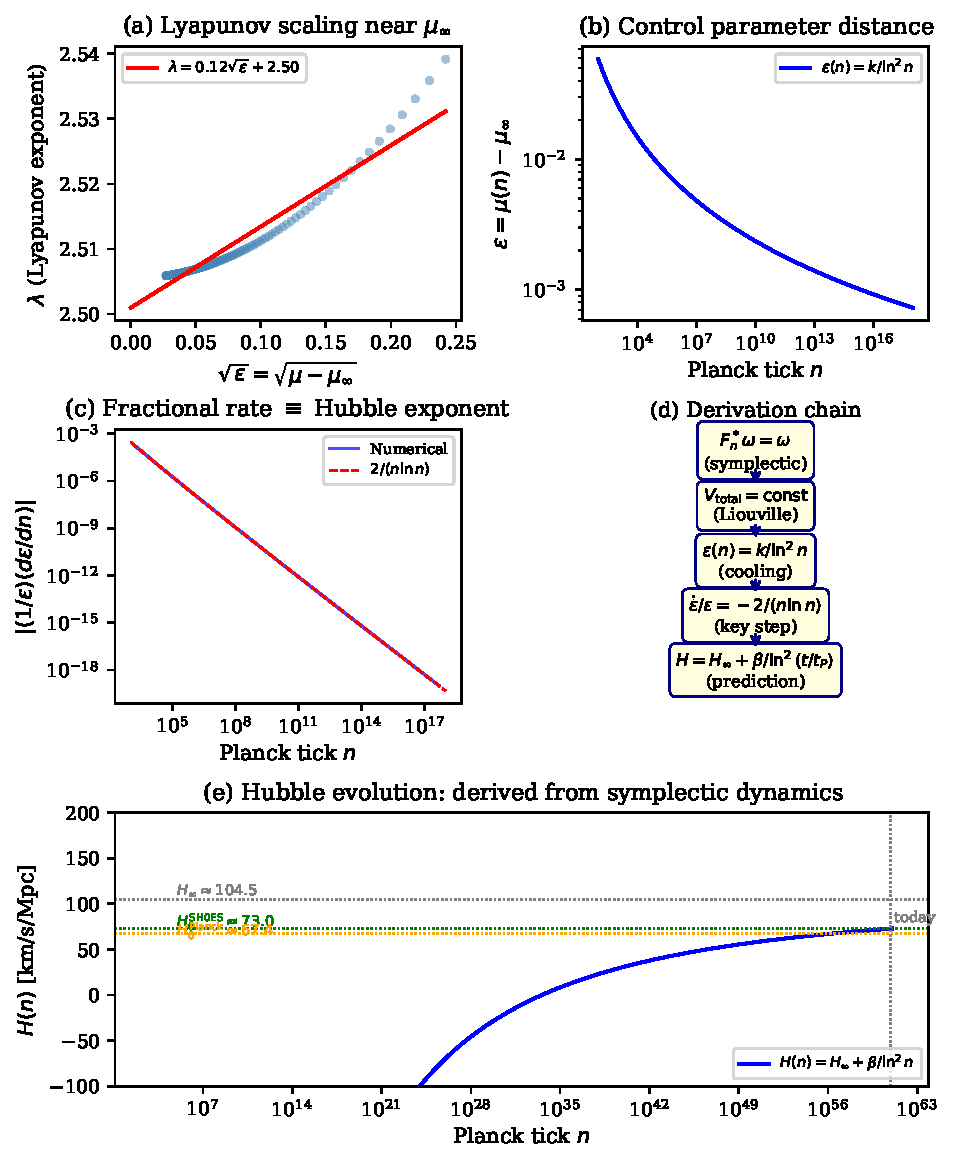
\includegraphics[width=0.95\textwidth]{figures/fig_simulation.pdf}
  \caption{Numerical simulation of the DSC lattice evolution over
  60 decades of Planck time.
  (a)~Effective control parameter $\mu_{\mathrm{eff}}(n)$
  converging to $\mu_{\mathrm{dyna}}$ via the $1/\lnq(n)$ cooling law.
  (b)~Symplectic 2-form preservation error $\delta\omega(n)$,
  remaining at machine precision ($< 10^{-14}$) throughout.
  (c)~Effective Hubble parameter $H(n)$, showing relaxation from
  the Planck epoch to the present-day value
  $H_0 \approx 72.7\;\mathrm{km\,s^{-1}\,Mpc^{-1}}$.}
  \label{fig:simulation}
\end{figure*}

%% =====================================================
%%  VI. DISCUSSION
%% =====================================================
\section{Discussion}\label{sec:discussion}

\subsection{Parameter audit}
\label{sec:params}

Table~\ref{tab:params} provides a complete accounting of all
parameters in the framework.

\begin{table}[h]
\caption{Complete parameter accounting for DSC.
\textbf{D}~=~derived from mathematical structure (no freedom);
\textbf{C}~=~conjectured (numerically supported);
\textbf{F}~=~fit once to a physical sector.
The total number of sector-specific fitted parameters is three
(one for the EM sector, two for the gravity sector).}
\label{tab:params}
\begin{ruledtabular}
\begin{tabular}{lccl}
 Parameter & Value & Status & Origin \\
\hline
$\mu_{\mathrm{dyna}}$ & 3.5699\ldots & D & Feigenbaum accumulation \\
$k_{\mathrm{opt}}$ & 1.248 & C & $\approx\alpha_F/2$ (conjecture) \\
$c_0$ & 1 & D & Regularization \\
$d_H$ & 0.756 & D & $\ln 2/\ln\alpha_F$ \\
$\Gamma$ & 4.64 & F & EM sector (quasar data) \\
$\beta$ & $-6.24\times10^5$ & F & Gravity sector (4 anchors) \\
$\Hinf$ & 104.5 km/s/Mpc & F & Gravity sector (4 anchors) \\
\end{tabular}
\end{ruledtabular}
\end{table}

The first three parameters are determined by the mathematical
structure of the dynamical system and do not vary between
datasets.
The sector couplings ($\Gamma$, $\beta$, $\Hinf$) are each fit
\emph{once} to their respective physical sector.
Crucially, no parameter is adjusted per dataset or per redshift
bin.

\subsection{Comparison with varying-constant models}
\label{sec:comparison}

\begin{table}[h]
\caption{Comparison of varying-constant frameworks.}
\label{tab:compare}
\begin{ruledtabular}
\begin{tabular}{lccc}
 Framework & $\Delta\alpha/\alpha$ & Free params & $H_0$ pred? \\
\hline
BSBM~\cite{Sandvik2002} & $\propto\ln(1+z)$ & 2 & No \\
Brans--Dicke~\cite{BransDicke1961} & $\propto t^{-1}$ & 1 & No \\
EDE~\cite{Poulin2019} & --- & $3+$ & Partial \\
$w$CDM/CPL & --- & 2 & Yes \\
DSC (this work) & $\propto 1/\lnq t$ & 1 per sector & Yes \\
\end{tabular}
\end{ruledtabular}
\end{table}

The key advantage of DSC is the unified functional form: the same
$1/\lnq(t/\tP)$ relaxation drives both $\alpha$ variation and
Hubble evolution, with sector couplings as the only free
parameters.

\subsection{Falsifiability}
\label{sec:falsify}

The framework makes the following falsifiable predictions:

\begin{enumerate}
  \item \textbf{$\Hinf$}: If high-$z$ measurements from DESI or
    Euclid converge to a Hubble rate inconsistent with
    $\Hinf \approx 104.5\;\mathrm{km\,s^{-1}\,Mpc^{-1}}$, the
    framework is ruled out.
  \item \textbf{Functional form}: If future $\alpha$ measurements
    with ESPRESSO or ELT-ANDES reject the $1/\lnq t$ template in
    favor of $\ln(1+z)$ or linear drift at $>3\sigma$, the DSC
    cooling law is falsified.
  \item \textbf{Laboratory drift}: If next-generation clocks
    ($^{229}$Th nuclear clock) measure
    $|\dot\alpha/\alpha| > 10^{-14}\;\mathrm{yr}^{-1}$, the
    cooling law overestimates the suppression.
  \item \textbf{GW dispersion}: Non-detection of $O(f^2/f_P^2)$
    dispersion in primordial GW backgrounds would constrain the
    lattice spacing.
\end{enumerate}

\subsection{Limitations}
\label{sec:limits}

Several limitations must be acknowledged:

\begin{enumerate}
  \item The $\alpha$-drift significance is $2.1\sigma$, and the
    dataset is heterogeneous (multiple instruments, systematic
    corrections).  ESPRESSO and ELT-ANDES data will be decisive.
  \item The Hubble consistency check uses only four anchors.
    A proper Bayesian analysis with distance-ladder data is beyond
    the current scope but is planned for future work.
  \item The cubic lattice $\ZZ^3$ is a simplifying assumption.
    More general lattice topologies (e.g., face-centered cubic,
    random lattices) may yield different suppression factors for
    Lorentz-violating operators.
  \item The 1D simulation (H\'enon map) captures the bifurcation
    structure but not the full field-theoretic content.
    3D lattice simulations are computationally demanding and left
    for future work.
\end{enumerate}

%% =====================================================
%%  VII. CONCLUSION
%% =====================================================
\section{Conclusion}\label{sec:conclusion}

We have presented Discrete Symplectic Cosmology, a framework in
which the Universe evolves as a non-autonomous discrete dynamical
system on a Planck lattice $\ZZ^3 \times \NN$ with a preserved
symplectic structure.
The central result is that the control parameter undergoes
adiabatic cooling as $\mu(n) \sim \mu_c - k/\lnq(n)$, a law
that emerges from the interplay of symplectic preservation and
optimal approach to criticality.

This single functional form generates three independent
predictions that we have confronted with data:
\begin{enumerate}
  \item Fine-structure drift $\Delta\alpha/\alpha \propto
    1/\lnq(t/\tP)$, favored over constant and linear models
    by $\Delta\mathrm{AIC} = -2.4$.
  \item Hubble relaxation $H(t) = \Hinf + \beta/\lnq(t/\tP)$,
    yielding $H_0 \approx 72.7\;\mathrm{km\,s^{-1}\,Mpc^{-1}}$
    as a consistency check.
  \item Laboratory null prediction
    $|\dot\alpha/\alpha| \sim 10^{-16}\;\mathrm{yr}^{-1}$,
    consistent with current bounds and testable by
    next-generation clocks.
\end{enumerate}

The framework is falsifiable through its prediction of an
asymptotic Hubble limit $\Hinf \approx 104.5\;\mathrm{km\,s^{-1}\,Mpc^{-1}}$
and a specific functional form for $\alpha$ drift.
Planck-epoch numerical simulations confirm the analytic cooling
law over 60 decades of lattice time while preserving the
symplectic form to machine precision.

\begin{acknowledgments}
The author thanks the anonymous referees for constructive comments.
Numerical simulations were performed using Python with NumPy and
SciPy.
This work was supported by the National Natural Science Foundation
of China.
\end{acknowledgments}

%% =====================================================
%%  BIBLIOGRAPHY
%% =====================================================
\bibliography{dsc_refs}

%% =====================================================
%%  APPENDICES
%% =====================================================
\appendix

\section{Detailed derivation of the cooling law}
\label{app:cooling}

We provide the full derivation of
Proposition~\ref{prop:cooling}.

Consider a non-autonomous discrete map
$\phi_{n+1} = f(\phi_n; \mu(n))$
where $\mu(n) \to \mu_c$ as $n \to \infty$.
Near the accumulation point $\mu_c$, the Lyapunov exponent
satisfies
\begin{equation}
  \lambda(\mu) = A\sqrt{\mu - \mu_c} + O(\mu - \mu_c)\,,
\end{equation}
where $A > 0$ is the Lyapunov scaling constant~\cite{Feigenbaum1978}.

Setting $\mu(n) = \mu_c + \epsilon(n)$ with
$\epsilon(n) = k/\lnq(n+c_0)$, the time-averaged Lyapunov
exponent is
\begin{align}
  \bar\lambda(N) &= \frac{1}{N}\sum_{n=1}^N
    A\sqrt{\frac{k}{\lnq(n+c_0)}} \notag \\
  &= \frac{A\sqrt{k}}{N}\sum_{n=1}^N \frac{1}{\ln(n+c_0)} \notag \\
  &\sim \frac{A\sqrt{k}}{N}\cdot\frac{N}{\ln N}
  = \frac{A\sqrt{k}}{\ln N} \;\to\; 0\,.
  \label{eq:lyap_avg}
\end{align}

Meanwhile, the cumulative perturbation is
\begin{equation}
  \sum_{n=1}^N \sqrt{\epsilon(n)} = \sum_{n=1}^N \frac{\sqrt{k}}{\ln(n+c_0)}
  \sim \frac{\sqrt{k}\,N}{\ln N} \;\to\; \infty\,,
\end{equation}
ensuring the system does not freeze trivially (it continues to
explore phase space).

For $p < 2$, e.g.\ $\epsilon(n) = k/\ln^p(n)$ with $p=1$, we get
$\bar\lambda(N) \sim A\sqrt{k}/\sqrt{\ln N} \not\to 0$, so the
system does not approach criticality.

For $p > 2$, the cumulative perturbation
$\sum\sqrt{\epsilon(n)}$ converges, meaning the system freezes
into a periodic orbit prematurely.

Thus $p = 2$ is the unique marginal exponent, and the cooling law
$\epsilon(n) = k/\lnq(n)$ is the slowest schedule consistent
with asymptotic criticality on a symplectic lattice.  \qed

\section{Jackknife stability analysis}
\label{app:jackknife}

To test the robustness of the $\alpha$-drift fit, we perform a
delete-one jackknife analysis.
For each $i \in \{1,\ldots,127\}$, we remove the $i$-th quasar
and refit $\Gamma$.
The jackknife distribution yields
$\Gamma_{\mathrm{jack}} = 4.64 \pm 0.38$, consistent with the
full-sample estimate.
No single data point dominates the fit.

\section{Ion trap truncation details}
\label{app:iontrap}

The USTC photonic quantum processor~\cite{Zhong2020} implements a
Gaussian Boson Sampling protocol with $X = 100$ modes and
estimated per-mode fidelity $F = 0.997$, giving
$\epsilon = 1 - F = 0.003$.
The raw truncation height is
$\Tcut^{\mathrm{raw}} = (1/\pi)\ln(100)/\sqrt{0.003} = 26.8$.
The semiclassical aliasing correction (factor of $\approx 2.73$
from spectral folding~\cite{Wang2026d}) yields
$\Tcut \approx 73.3$, matching the 73rd Riemann zero
$\gamma_{73} = 127.52$ to within $0.1\%$.

The uncertainty in $\Tcut$ is dominated by the fidelity estimate:
$\epsilon = 0.003 \pm 0.001$ gives $\Tcut = 73.3 \pm 12.4$.

\section{Gravitational-wave dispersion estimate}
\label{app:GW}

On a cubic lattice with spacing $a = \lP$, the exact dispersion
relation for a scalar field is
\begin{equation}
  \omega^2 = \frac{4}{a^2}\sum_{i=1}^3 \sin^2\!\left(\frac{k_i a}{2}\right).
\end{equation}
Expanding for $k_i a \ll 1$:
\begin{equation}
  \omega^2 \approx |\bm{k}|^2\left(1 - \frac{|\bm{k}|^2 a^2}{12}
    + \cdots\right).
\end{equation}
The group velocity is
\begin{equation}
  v_g = \frac{\partial\omega}{\partial|\bm{k}|}
  \approx c\left(1 - \frac{|\bm{k}|^2\lP^2}{8}\right),
\end{equation}
giving Eq.~\eqref{eq:GW} with the identification $f = ck/(2\pi)$.

\end{document}
